% ===========================================================================
\section{Desenvolvimento e implementa\c{c}\~ao}
\label{sec:desenvolvimento}
% ===========================================================================

A constru\c{c}\~ao do modelo vive em tr\^es \emph{scripts} independentes do estado da
cena --- um de \emph{build}, um de verifica\c{c}\~ao e um de galeria --- mais uma biblioteca de
\emph{helpers} compartilhada. Esta se\c{c}\~ao descreve as decis\~oes de implementa\c{c}\~ao
que sustentam os resultados da Se\c{c}\~ao~\ref{sec:resultados}.

\subsection{Organiza\c{c}\~ao do c\'odigo e idempot\^encia}

O \emph{script} de \emph{build} limpa integralmente a cena --- objetos, materiais e dados
\'orf\~aos --- antes de reconstru\'i-la. Essa idempot\^encia \'e o que permite trat\'a-lo como
a fonte da verdade: qualquer estado que n\~ao possa ser reproduzido pelo \emph{script}
simplesmente n\~ao sobrevive \`a pr\'oxima execu\c{c}\~ao. Duas salvaguardas acompanham essa
disciplina. A primeira \'e a detec\c{c}\~ao da raiz do projeto por verifica\c{c}\~ao de
marcadores (\texttt{images/} e \texttt{scripts/lotus\_common.py}), porque o diret\'orio de
trabalho do Blender n\~ao coincide necessariamente com o do reposit\'orio. A segunda \'e o
recarregamento expl\'icito do m\'odulo de \emph{helpers} a cada \emph{build}: em sess\~oes
longas, o m\'odulo permanece em cache e misturaria vers\~oes distintas do c\'odigo.

\subsection{Biblioteca de \emph{helpers}}

A biblioteca concentra quatro grupos de fun\c{c}\~oes. O primeiro constr\'oi malhas: um
gerador de \emph{loft} por encadeamento de an\'eis, um gerador de superf\'icies de
revolu\c{c}\~ao, primitivas param\'etricas (caixa chanfrada, cilindro, setor de anel) e a
tampa descrita adiante. O segundo trata materiais. O terceiro mede malhas --- v\'ertices,
faces por tipo, arestas n\~ao variedade, arestas de borda --- e o envelope de cena. O quarto
grava metadados nos objetos.

Duas fun\c{c}\~oes merecem destaque por sua rela\c{c}\~ao com as restri\c{c}\~oes do projeto.
A primeira \'e a convers\~ao de espa\c{c}\~o de cor, que aplica a transforma\c{c}\~ao n\~ao
linear de sRGB para linear a cada canal; todas as cores do modelo passam por ela, o que
elimina a classe de erro discutida na Se\c{c}\~ao~\ref{sec:fundamentacao}. A segunda \'e a
sele\c{c}\~ao de n\'os por identificador de tipo (\texttt{bl\_idname}) em vez de nome
exibido: como a interface do Blender \'e traduzida, buscar um n\'o pelo r\'otulo na
interface em portugu\^es falha silenciosamente. No c\'odigo, a refer\^encia \'e sempre
\texttt{ShaderNodeBsdfPrincipled}, e n\~ao o texto exibido.

\subsection{Materiais}

Treze materiais comp\~oem a cena. O principal \'e a pintura azul multicamada, com cor base
definida em sRGB e convertida para linear, perturba\c{c}\~ao de alta frequ\^encia nos canais
de rugosidade, metalicidade e normal --- o que produz a leitura de micro-flocos apenas em
closes, como previsto na especifica\c{c}\~ao --- e camada de verniz com
\'indice de refra\c{c}\~ao 1,55 e rugosidade 0,02. Os doze restantes cobrem borracha,
policarbonato de far\'ois e lanternas, metais (alum\'inio escovado, cromo, a\c{c}o
escurecido), tecido do interior e vidro.

A refra\c{c}\~ao por tra\c{c}ado de raios \'e habilitada explicitamente nos materiais
transparentes. Sem essa habilita\c{c}\~ao, o efeito n\~ao aparece no motor de tempo real
utilizado, mesmo que a transmiss\~ao esteja configurada \cite{blender5manual}.

\subsection{O casco principal}

\subsubsection{Perfil transversal}

O perfil de meio-lado tem nove pontos, definidos por sete par\^ametros: meia-largura
m\'axima $w$, meia-largura do topo $w_t$, cota do fundo $z_b$, cota do ombro $z_s$, cota da
aresta superior $z_{te}$ e cota do centro do topo $z_t$. A fun\c{c}\~ao espelha o
meio-perfil e fecha o la\c{c}o, resultando em dezesseis pontos por anel. A ordem dos pontos
\'e significativa: ela define a dire\c{c}\~ao das cadeias de arestas que percorrem o casco
no sentido longitudinal e, portanto, o fluxo de arestas do modelo. Os pontos que concentram
a inflex\~ao de largura m\'axima e o ombro s\~ao as regi\~oes de maior curvatura e as que
mais influenciam a leitura da silhueta.

\subsubsection{Esta\c{c}\~oes}

O casco \'e definido por 47 esta\c{c}\~oes transversais, cada uma com sua s\'extupla
$(x, w, w_t, z_s, z_{te}, z_t)$; a cota do fundo \'e calculada, e n\~ao tabelada, porque
depende dos v\~aos de roda. Tr\^es caracter\'isticas merecem leitura. Primeiro, a largura
m\'axima ocorre pr\'oximo ao eixo traseiro ($w = 0{,}859$\,m em $x = -1{,}150$), o que
reproduz a distribui\c{c}\~ao de massa visual do ve\'iculo real, com a traseira mais larga
que a dianteira. Segundo, a cota do topo cresce de $0{,}592$\,m no nariz at\'e
$0{,}911$\,m no \emph{deck}, evidenciando a inclina\c{c}\~ao ascendente da superf\'icie.
Terceiro, h\'a esta\c{c}\~oes repetidas no nariz ($1{,}863$ e $1{,}856$\,m) e na cauda
($-1{,}852$ e $-1{,}858$\,m): s\~ao an\'eis de reten\c{c}\~ao, discutidos adiante.

\subsubsection{Arcos de roda sem opera\c{c}\~oes booleanas}

O recorte do arco \'e obtido por c\'alculo, e n\~ao por subtra\c{c}\~ao. Para cada
esta\c{c}\~ao, a cota do fundo \'e a maior entre a cota base da carroceria e a
circunfer\^encia de cada arco:

\begin{lstlisting}[language=Python]
def arch_bottom(x, base, arches) -> float:
    """Body bottom accounting for wheel arches."""
    z = base
    for x_axle, z_axle, radius in arches:
        dx = x - x_axle
        if abs(dx) < radius:
            z = max(z, z_axle + math.sqrt(radius * radius - dx * dx))
    return z
\end{lstlisting}

Os par\^ametros s\~ao $(x_{\text{eixo}}, z_{\text{eixo}}, r)$ para cada arco: dianteiro com
raio $0{,}335$\,m e traseiro com raio $0{,}350$\,m, ambos centrados na cota do raio do pneu
correspondente. A eleva\c{c}\~ao do fundo nas esta\c{c}\~oes pr\'oximas ao eixo produz o
``t\'unel'' do arco sem qualquer altera\c{c}\~ao na conectividade da malha, o que preserva a
grade quadrangular e a continuidade dos reflexos sobre o para-lama.

\subsubsection{Tampas de extremidade}

Fechar o nariz e a cauda \'e o ponto em que a maioria das implementa\c{c}\~oes ing\^enuas
introduz n-gons: o contorno tem dezesseis v\'ertices, e preench\^e-lo com uma \'unica face
produziria um n-gon de dezesseis lados. A biblioteca implementa uma tampa por ``leque
dobrado'', em que cada quad conecta um par de v\'ertices consecutivos ao par espelhado do
lado oposto do la\c{c}o:

\begin{lstlisting}[language=Python]
def _folded_fan_cap(bm, verts, mat_index, smooth=True):
    """Cap a closed loop using quads only (even n)."""
    n = len(verts)
    if n < 4:
        return []
    if n % 2:
        n -= 1
    created = []
    for i in range(n // 2 - 1):
        a, b = verts[i], verts[i + 1]
        c, d = verts[n - 2 - i], verts[n - 1 - i]
        if len({a, b, c, d}) < 4:
            continue
        try:
            face = bm.faces.new((a, b, c, d))
        except ValueError:
            continue
        face.material_index = mat_index
        created.append(face)
    return created
\end{lstlisting}

A t\'ecnica tem uma consequ\^encia geom\'etrica que precisa ser compreendida: a tampa
resultante n\~ao \'e plana, e sim uma superf\'icie dobrada. Como a regi\~ao \'e levemente
curva e fica nas extremidades do ve\'iculo, o resultado \'e visualmente adequado e,
sobretudo, topologicamente limpo. A mesma fun\c{c}\~ao \'e reutilizada para eliminar tampas
n-gon geradas pelas primitivas de cilindro, o que unifica a garantia: qualquer face com mais
de quatro lados \'e substitu\'ida por quads antes de a malha ser convertida em objeto.

\subsubsection{An\'eis de reten\c{c}\~ao}

As esta\c{c}\~oes repetidas no nariz e na cauda s\~ao um recurso deliberado. Sob
subdivis\~ao, uma sequ\^encia de esta\c{c}\~oes muito espa\c{c}adas nas extremidades faz
com que a superf\'icie limite retraia e arredonde o contorno, produzindo aspecto de
``bal\~ao''. Inserir duas esta\c{c}\~oes quase coincidentes cria uma descontinuidade de
segunda ordem que ``segura'' o contorno, achatando a face terminal e estabilizando a
silhueta. O custo \'e de tr\^es faces por extremidade.

\subsubsection{Rebaixos reais}

Dois recortes s\~ao feitos por deslocamento direto de v\'ertices, com fun\c{c}\~ao de
atenua\c{c}\~ao suave. O primeiro opera apenas nos v\'ertices laterais e os desloca para
dentro segundo uma elipse, com profundidade m\'axima de 62\,mm. O expoente 1,5 na
fun\c{c}\~ao de atenua\c{c}\~ao foi escolhido para produzir uma transi\c{c}\~ao ligeiramente
mais r\'apida que a quadr\'atica, evitando uma borda excessivamente mole. O segundo recorte
--- o alojamento dos far\'ois --- usa a mesma estrat\'egia com atenua\c{c}\~ao c\^onica,
escavando 30\,mm no painel dianteiro em torno de duas elipses centradas em
$y = \pm0{,}470$\,m.

Vale registrar por que a alternativa foi descartada. A especifica\c{c}\~ao original pedia
que as aberturas de ventila\c{c}\~ao fossem geometria real, e n\~ao mapa de normais. A
escolha atende ao requisito e, adicionalmente, torna a profundidade do rebaixo um
par\^ametro num\'erico audit\'avel, em vez de um valor visualmente estimado.

\subsection{Cabine, rodas e conjuntos \'opticos}

A cabine \'e um segundo \emph{loft} assentado sobre a linha de cintura, com perfil de dez
pontos, topo plano e laterais quase verticais --- geometria de \emph{hardtop} r\'igido. O
material de vidro \'e atribu\'ido por \emph{faixa de faces} no pr\'oprio \emph{loft}, e
n\~ao por placas adicionais: assim o vidro n\~ao \'e uma superf\'icie flutuante sobre a
carroceria, mas parte do mesmo corpo cont\'inuo. O interior \'e simplificado por decis\~ao
de escopo, com assentos, painel, volante e arco de seguran\c{c}a.

As quatro rodas s\~ao geradas por uma \'unica fun\c{c}\~ao parametrizada --- revolu\c{c}\~ao
de perfil para o pneu, seis raios, disco e pin\c{c}a de freio --- variando apenas o raio. Os
pneus seguem as designa\c{c}\~oes 185/55R15 (dianteiro) e 205/50R16 (traseiro). Essa
parametriza\c{c}\~ao \'e o exemplo mais claro de geometria em que a automa\c{c}\~ao por
c\'odigo tem vantagem evidente: 52 objetos de roda saem de uma fun\c{c}\~ao, enquanto o
casco --- um \'unico objeto --- exigiu a maior parte do esfor\c{c}o de itera\c{c}\~ao.

Os conjuntos \'opticos dianteiros comb\~em carca\c{c}a, refletor e lente de policarbonato,
com dois far\'ois auxiliares circulares; a traseira tem quatro lanternas redondas com aro
met\'alico. Os emblemas \texttt{LOTUS}, \texttt{111S} e o frontal s\~ao malha real,
produzida a partir de glifos de texto convertidos em geometria.

\subsection{Nomenclatura, metadados e subdivis\~ao}

Todo objeto recebe um prefixo de categoria --- \texttt{GEO\_} para geometria, \texttt{LGT\_}
para luzes, \texttt{CAM\_} para c\^ameras --- e cada objeto de geometria recebe tr\^es
propriedades personalizadas: \texttt{cat}, \texttt{part} e \texttt{mat\_swap\_key}. O
objetivo declarado \'e permitir troca automatizada de material: um agente pode localizar
todos os objetos cujo \texttt{mat\_swap\_key} seja \texttt{paint\_primary} e substituir o
material sem inspecionar nomes de objeto. \'E um exemplo de como a conven\c{c}\~ao de
nomenclatura deixa de ser est\'etica e passa a ser uma interface de programa\c{c}\~ao.

Os dois corpos principais recebem o modificador de subdivis\~ao com n\'ivel de
visualiza\c{c}\~ao 1 e n\'ivel de render 3. A assimetria \'e deliberada: o n\'ivel 3 no
render garante a suavidade do resultado final, enquanto o n\'ivel 1 na visualiza\c{c}\~ao
mant\'em a resposta da interface utiliz\'avel.

\subsection{Relat\'orio de malha}

O \emph{build} termina emitindo um relat\'orio em formato de texto, com uma linha por objeto
e totais consolidados, contendo: v\'ertices, faces, quads, tri\^angulos e n-gons por objeto;
arestas n\~ao variedade; arestas de borda; e o envelope dimensional com a diferen\c{c}a em
rela\c{c}\~ao aos alvos.

O envelope \'e calculado varrendo os oito cantos da caixa delimitadora de cada objeto de
malha, transformados para coordenadas de mundo. A escolha de medir a caixa delimitadora dos
objetos, e n\~ao os v\'ertices da malha de controle, \'e relevante: o que define o envelope
percebido \'e a geometria \emph{avaliada}, j\'a subdividida, e n\~ao a malha de
controle.

\subsection{Configura\c{c}\~ao de render e mudan\c{c}as de API}

A configura\c{c}\~ao de render \'e feita por c\'odigo e precisa acomodar mudan\c{c}as
introduzidas nas vers\~oes recentes do Blender. Tr\^es delas afetam diretamente este projeto.

A primeira \'e a aus\^encia da \'arvore de composi\c{c}\~ao como propriedade da cena: o
compositor passou a ser um grupo de n\'os criado separadamente e associado \`a cena, e o
n\'o de sa\'ida \texttt{Composite} foi substitu\'ido por um n\'o de sa\'ida de grupo. A
segunda \'e a aus\^encia do efeito de brilho no motor: o brilho passou a ser obtido por um
n\'o de \emph{glare} no compositor. A terceira s\~ao os nomes v\'alidos do \emph{look} de
mapeamento de tons, que variam entre vers\~oes e cujo nome inv\'alido interrompe a
execu\c{c}\~ao; a solu\c{c}\~ao adotada \'e uma tentativa em cascata.

O padr\~ao \'e sempre o mesmo: verificar a exist\^encia do atributo antes de us\'a-lo e
falhar de forma tolerante. Em um contexto de automa\c{c}\~ao por agente, essa disciplina tem
valor adicional --- uma exce\c{c}\~ao n\~ao tratada interrompe a sess\~ao e obriga a um novo
ciclo de diagn\'ostico, enquanto uma degrada\c{c}\~ao controlada mant\'em o
\emph{pipeline} execut\'avel. Uma armadilha de natureza diferente foi verificada: a
atribui\c{c}\~ao de escala a um objeto exige uma tupla de tr\^es elementos, e
constru\c{c}\~oes que produzem tuplas de tamanho vari\'avel n\~ao s\~ao aceitas. \'E um erro
que s\'o se manifesta em tempo de execu\c{c}\~ao dentro do Blender.

\subsection{O ciclo de chamadas via MCP}

A opera\c{c}\~ao por MCP reduz o ciclo de trabalho a tr\^es ferramentas: executar
c\'odigo, consultar a cena e capturar a imagem da \emph{viewport}
(Figura~\ref{fig:sequencia}). O encadeamento tem uma propriedade importante: a mensagem de
execu\c{c}\~ao \'e, ela pr\'opria, o artefato de reprodutibilidade. Executar o mesmo
\emph{script} por linha de comando ou por MCP produz a mesma cena, porque nos dois casos o
que se executa \'e o mesmo c\'odigo; a diferen\c{c}a est\'a no \emph{registro}. No modo MCP,
argumentos e resultados ficam serializados como mensagens do protocolo; no modo linha de
comando, restam no hist\'orico do terminal.

\begin{figure}[htbp]
  \centering
  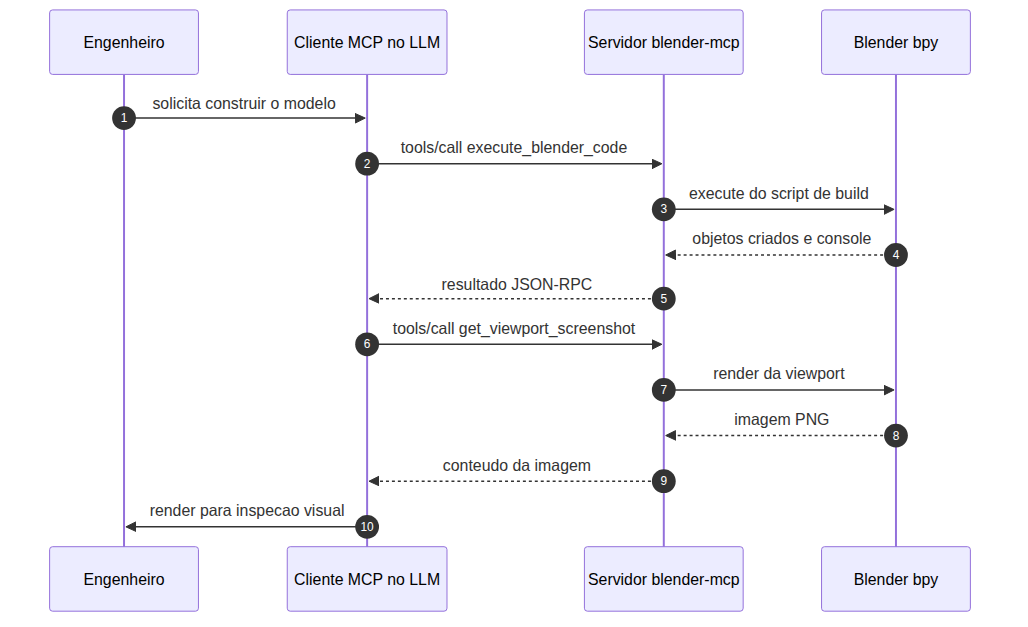
\includegraphics[width=0.90\textwidth]{figures/sequencia-build.png}
  \caption{Ciclo de chamadas do protocolo durante um ciclo de constru\c{c}\~ao e
           inspe\c{c}\~ao. Cada chamada \'e uma mensagem serializada, o que constitui o
           registro audit\'avel do processo.}
  \label{fig:sequencia}
  \fonte{elaborado pelo autor (2026).}
\end{figure}

A galeria de apresenta\c{c}\~ao usa um \emph{rig} distinto e tempor\'ario --- luzes de
recorte laterais, emiss\~ao nos elementos \'opticos e brilho no compositor --- e
\emph{n\~ao} grava o arquivo de cena. A decis\~ao \'e deliberada: o \emph{rig} dram\'atico
\'e um artefato de apresenta\c{c}\~ao, e n\~ao um estado do modelo; persist\'i-lo
contaminaria o ambiente de verifica\c{c}\~ao e quebraria a reprodutibilidade dos renders
neutros. A Figura~\ref{fig:galeria-luz} mostra o resultado.

\begin{figure}[htbp]
  \centering
  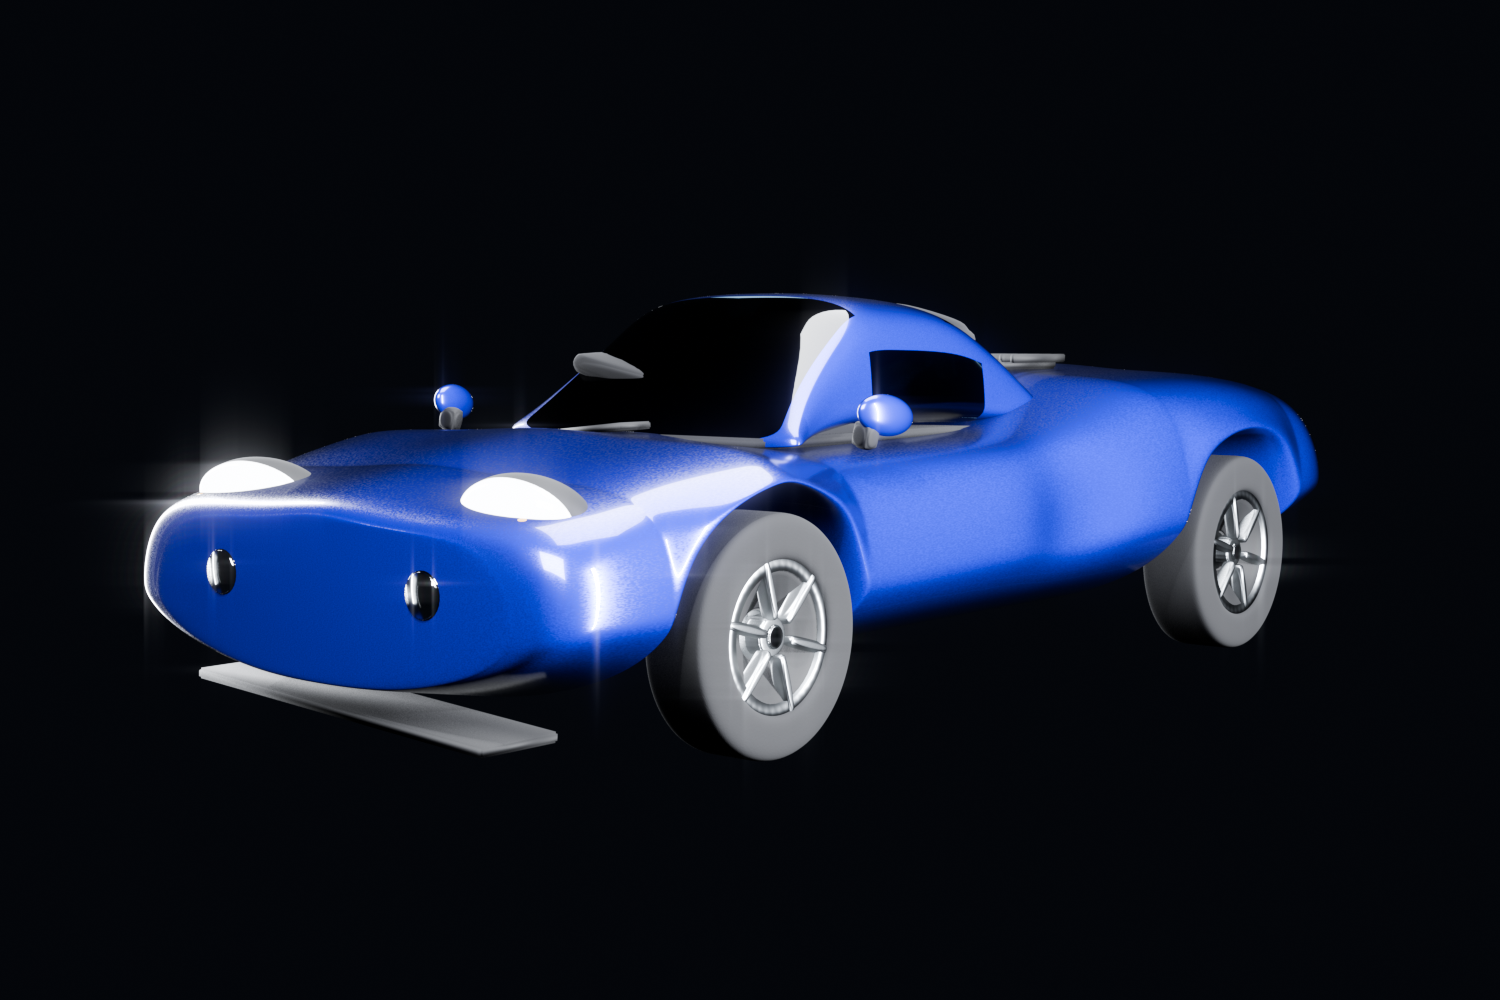
\includegraphics[width=0.80\textwidth]{figures/gal-luz.png}
  \caption{Imagem de apresenta\c{c}\~ao com \emph{rig} dram\'atico tempor\'ario: luzes de
           recorte laterais, elementos \'opticos acesos e brilho via n\'o de \emph{glare}.
           O \emph{rig} n\~ao \'e persistido no arquivo de cena.}
  \label{fig:galeria-luz}
  \fonte{elaborado pelo autor (2026).}
\end{figure}
